\documentclass[aspectratio=43]{beamer}
\beamertemplatenavigationsymbolsempty

\mode<presentation>
{
	\usetheme{Singapore}
        \useoutertheme{miniframes}
	%\setbeamercovered{transparent}
	%\setbeamertemplate{footline}[]
        \setbeamertemplate{footline}
                          {
                            \leavevmode%
                            \hbox{%
                              \begin{beamercolorbox}[wd=.333333\paperwidth,ht=2.25ex,dp=1ex,center]{author in head/foot}%
                                \usebeamerfont{author in head/foot}\insertauthor
                              \end{beamercolorbox}%
                              \begin{beamercolorbox}[wd=.333333\paperwidth,ht=2.25ex,dp=1ex,center]{title in head/foot}%
                                \usebeamerfont{title in head/foot}\insertshorttitle
                              \end{beamercolorbox}%
                              \begin{beamercolorbox}[wd=.333333\paperwidth,ht=2.25ex,dp=1ex,right]{date in head/foot}%
                                \usebeamerfont{date in head/foot}\insertshortdate{}\hspace*{2em}
                                \insertframenumber{} / \inserttotalframenumber\hspace*{2ex}
                            \end{beamercolorbox}}%
                            \vskip0pt%
                          }
}

% \usepackage{flashmovie}
\usepackage[utf8]{inputenc}
\usepackage[T1]{fontenc}
%\usepackage[ngerman]{babel}
\usepackage[english]{babel}
\usepackage{amsmath}
\usepackage[absolute,overlay]{textpos}
\usepackage{svg}
\usepackage{xcolor}

\usebackgroundtemplate{%
\begin{tikzpicture}[remember picture,overlay]
\node[anchor=south west] at (current page.south west) {\includegraphics[height=0.4cm]{by.eps}};
\end{tikzpicture}}

\author[]{Anton Kuzmin}
\institute[]{}
\date[FOSDEM 2024]{FOSDEM'24, 3 \& 4 February 2024, Brussels}

\usepackage{tikz}

\title{Cologne Chip GateMate FPGA -- filling a gap between hardware and software}

\setbeamerfont{table font}{size=\tiny}

\begin{document}

\begin{frame}
  \titlepage
\end{frame}

\section{Intro}

\begin{frame}
  \frametitle{Who am I\dots}
  \begin{itemize}
  \item not really a software developer\\
    \dots but write code sometimes
  \item developing embedded systems for 25 years
  \item VME, CompactPCI, AdvancedTCA, SoM
  \item FPGA and SoC-FPGA (Altera/Intel, Microsemi/Microchip, Cologne Chip)
  \item VHDL (RTL-code, no, it is not a software)
  \end{itemize}
  \vskip.5cm

%  My usual problem with the software is how to make it run on a
%  hardware which is known not to be working yet and how to bring-up
%  and test this hardware. With a soft-core CPU it is getting even
%  worse.

\end{frame}


\frame{\tableofcontents[subsectionstyle=show]}

\section{FPGA and software}

\begin{frame}
\frametitle{Why software develpers should care about FPGA}
\end{frame}

\begin{frame}
\frametitle{Current state (for 40 years)}
% tabulator control pannel -- hardwiring
% strictly cross
\end{frame}

\section{Self-hosted FPGA}

% Native vs Na\"ive

\begin{frame}
\frametitle{Demo\dots}
\end{frame}

\begin{frame}
\frametitle{Perspectives}
\end{frame}

\section{Cologne Chip GateMate FPGA}

\begin{frame}
\frametitle{Overview}
\end{frame}

\begin{frame}
\frametitle{CPE}
\end{frame}

\begin{frame}
\frametitle{GMM-7550}
\end{frame}

\section{What's next}

\begin{frame}
\frametitle{Challenges ahead}
\begin{itemize}
  \item \textbf{integration}
\end{itemize}
\end{frame}

\begin{frame}
\frametitle{It doesn't have to be\dots}
% CTA
\end{frame}

\section{Contact info}
\begin{frame}

  \begin{minipage}{7cm}
    \vskip.5cm
    \huge{Thank you!}
    \vskip1cm
    \small{Anton Kuzmin}\\
    \small{\texttt{ak@gmm7550.dev}}\\
    \small{\texttt{https://github.com/gmm-7550/}}
    \vskip.5cm
    \Huge{Questions?..}
  \end{minipage}

  \vspace{-5cm}
  \begin{flushright}
    \includegraphics[height=5cm]{gmm7550-vcard.png}\\
  \end{flushright}

\end{frame}


\end{document}
